% Silver Cooks - Book Cover
% With proper RTL support

\documentclass[tikz]{standalone}
\usepackage{fontspec}
\usepackage{xcolor}
\usepackage{graphicx}
\usepackage{luabidi}

% Fonts
\setmainfont{Helvetica Neue}
\newfontfamily\titlefont{Palatino}
\newfontfamily\hebrewfont[Script=Hebrew]{Arial Hebrew}
\newfontfamily\arabicfont[Script=Arabic]{Geeza Pro}
\newfontfamily\spanishfont{Georgia}

% RTL commands
\newcommand{\heb}[1]{{\hebrewfont\RL{#1}}}
\newcommand{\arb}[1]{{\arabicfont\RL{#1}}}

% Colors from cookbook
\definecolor{bgpage}{HTML}{FAF6F1}
\definecolor{ink}{HTML}{222222}
\definecolor{muted}{HTML}{777777}
\definecolor{accent}{HTML}{D9925B}

\begin{document}
\begin{tikzpicture}[x=1in, y=1in]

% === BACKGROUND IMAGE ===
\node[anchor=south west, inner sep=0pt] at (0,0) {
  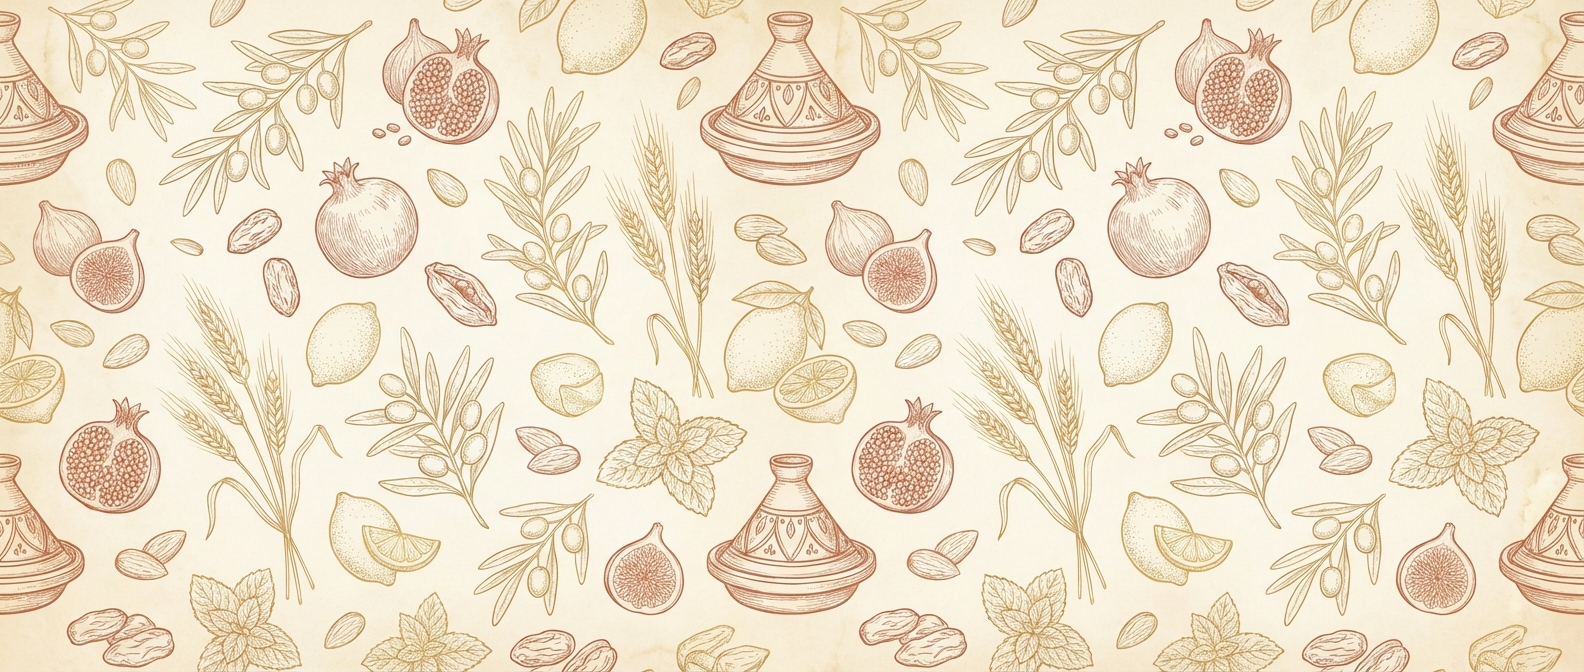
\includegraphics[width=16.95in, height=8.25in]{background.png}
};

% === PAGE COLOR OVERLAY ===
\fill[bgpage, opacity=0.92] (0,0) rectangle (16.95, 8.25);

% ========================================
% BACK COVER (center at x=4.125)
% ========================================

% Book titles - Hebrew and Arabic with RTL
\node[text=ink] at (4.125, 6.5) {
  \fontsize{18pt}{18pt}\selectfont
  \heb{מטבח מצפון}
  \hspace{0.4in}
  \arb{مطبخ بالأصل}
};

\node[text=ink] at (4.125, 5.9) {
  {\titlefont\fontsize{16pt}{16pt}\selectfont Oriented Kitchen}
  \hspace{0.3in}
  {\spanishfont\fontsize{14pt}{14pt}\selectfont\itshape Cocina con Conciencia}
};

% Subtitles
\node[text=muted, text width=5.5in, align=center] at (4.125, 4.9) {
  \fontsize{9pt}{15pt}\selectfont
  Plant-Based Recipes from Djerba \& Tangier\\[2pt]
  {\spanishfont\itshape Recetas a Base de Plantas de Djerba y Tánger}\\[2pt]
  \heb{מתכונים מבוססי צמחים מג׳רבה וטנג׳יר}\\[2pt]
  \arb{وصفات نباتية من جربة وطنجة}
};

% Divider
\draw[accent, line width=1pt] (2.5, 4.1) -- (5.75, 4.1);

% Recipe count
\node[text=ink] at (4.125, 3.6) {
  \fontsize{11pt}{11pt}\selectfont
  81 Recipes in Four Languages
};

% Website
\node[text=accent] at (4.125, 1.0) {
  \fontsize{10pt}{10pt}\selectfont
  silvercooks.com
};

% ========================================
% SPINE (8.125 to 8.825)
% ========================================
\fill[accent] (8.125, 0) rectangle (8.825, 8.25);

\node[rotate=90, text=bgpage] at (8.475, 4.125) {
  \fontsize{10pt}{10pt}\selectfont
  {\titlefont\bfseries Oriented Kitchen} \hspace{0.6em} \heb{מטבח מצפון} \hspace{0.6em} David \& Enny Silver
};

% ========================================
% FRONT COVER (center at x=12.89)
% ========================================

% Row 1: Hebrew (right-aligned) + Arabic (left side)
\node[text=ink, anchor=east] at (12.5, 6.3) {
  \fontsize{28pt}{28pt}\selectfont
  \heb{מטבח מצפון}
};
\node[text=ink, anchor=west] at (13.3, 6.3) {
  \fontsize{24pt}{24pt}\selectfont
  \arb{مطبخ بالأصل}
};

% Row 2: English + Spanish
\node[text=ink, anchor=east] at (12.5, 5.4) {
  \titlefont\fontsize{24pt}{24pt}\selectfont
  Oriented Kitchen
};
\node[text=accent, anchor=west] at (13.3, 5.4) {
  \spanishfont\fontsize{18pt}{18pt}\selectfont\itshape
  Cocina con Conciencia
};

% Subtitles block
\node[text=muted, text width=6in, align=center] at (12.89, 4.4) {
  \fontsize{10pt}{16pt}\selectfont
  Plant-Based Recipes from Djerba \& Tangier\\[2pt]
  {\spanishfont\itshape Recetas a Base de Plantas de Djerba y Tánger}\\[2pt]
  \heb{מתכונים מבוססי צמחים מג׳רבה וטנג׳יר}\\[2pt]
  \arb{وصفات نباتية من جربة وطنجة}
};

% Divider
\draw[accent, line width=1.5pt] (10.5, 3.5) -- (15.28, 3.5);

% Family lines
\node[text=ink] at (12.89, 3.0) {
  \fontsize{11pt}{11pt}\selectfont
  Cohen-Trabelsi · \heb{כהן-טרבלסי} · \arb{كوهين-طرابلسي}
};
\node[text=muted] at (12.89, 2.6) {
  \fontsize{9pt}{9pt}\selectfont
  Djerba, Tunisia · \heb{ג׳רבה, תוניסיה} · \arb{جربة، تونس}
};

\node[text=ink] at (12.89, 2.0) {
  \fontsize{11pt}{11pt}\selectfont
  Kadoch-Muyal · \heb{קדוש-מויאל} · \arb{قدوش-مويال}
};
\node[text=muted] at (12.89, 1.6) {
  \fontsize{9pt}{9pt}\selectfont
  Tangier, Morocco · \heb{טנג׳יר, מרוקו} · \arb{طنجة، المغرب}
};

% Divider
\draw[accent, line width=1pt] (10.8, 1.15) -- (14.98, 1.15);

% Authors
\node[text=accent] at (12.89, 0.7) {
  \titlefont\fontsize{16pt}{16pt}\selectfont
  David \& Enny Silver
};

\end{tikzpicture}
\end{document}
